\clearpage
\section{Mask Coders Performance}
\label{secX:codersmask}

In this section we analyze the performance of every one of the mask coders implemented in Chapter \ref{coders}. Once again, the compression rate (equation~(\ref{eq:compression-rate})) and the relative difference (equation~(\ref{eq:relative-difference})) will be the metrics we use for comparing the coders between each other.

We considered the results obtained when coding the different data types of the datasets introduced in Chapter \ref{datasets}. For example, in Figure \ref{fig:mask-irkis} we can see the graphs obtained for the ``VWC" data type of the \datasetirkis \ dataset. For each <$\coder \in C$, $e \in E$> combination we plot two values: the window size which minimizes the compression rate and said compression rate.

Easily, after observing the plots we noticed that in general the compression rate for coders \textit{CoderPWLH-M}, \textit{CoderGAMPSLimit-M} and \textit{CoderSF-M} was worst than the rest.

Analyze the data and discard these 

PONER OTRA GRAFICA DE OTRO TIPO DE DATO

\clearpage


\newcommand{\legendsone}{
\begin{tabular}{| C{1.5cm} | C{1.5cm} | C{1.5cm} |}
\hline
  \multicolumn{1}{|>{\centering\arraybackslash}m{1.5cm}|}{\cpca PCA} 
& \multicolumn{1}{>{\centering\arraybackslash}m{1.5cm}|}{\capca APCA} 
& \multicolumn{1}{>{\centering\arraybackslash}m{1.5cm}|}{\cfr FR}\\
\toprule[0.1mm]
\end{tabular}
\vspace{+30pt}
}



\begin{sidewaystable}[ht]
\newcommand{\cgzip}{\cellcolor{orange!20}}
\newcommand{\cfr}{\cellcolor{yellow!25}}
\newcommand{\cpca}{\cellcolor{cyan!20}}
\newcommand{\capca}{\cellcolor{green!20}}
\centering

\legendsone

\begin{tabular}{| l | l | c | c || c | c || c | c || c | c || c | c || c | c || c | c || c | c |}
\cline{3-18}
\multicolumn{1}{c}{}& \multicolumn{1}{c|}{} & \multicolumn{2}{c||}{e = 0} & \multicolumn{2}{c||}{e = 1} & \multicolumn{2}{c||}{e = 3} & \multicolumn{2}{c||}{e = 5} & \multicolumn{2}{c||}{e = 10} & \multicolumn{2}{c||}{e = 15} & \multicolumn{2}{c||}{e = 20} & \multicolumn{2}{c|}{e = 30} \\\hline
{Dataset} & {Data Type} & {\footnotesize OWS} & {\footnotesize CR} & {\footnotesize OWS} & {\footnotesize CR} & {\footnotesize OWS} & {\footnotesize CR} & {\footnotesize OWS} & {\footnotesize CR} & {\footnotesize OWS} & {\footnotesize CR} & {\footnotesize OWS} & {\footnotesize CR} & {\footnotesize OWS} & {\footnotesize CR} & {\footnotesize OWS} & {\footnotesize CR} \\\hline\hline
{\datasetirkis} & {VWC} & {\capca4} & {\capca20.32} & {\capca4} & {\capca18.35} & {\capca5} & {\capca12.37} & {\capca6} & {\capca6.77} & {\capca7} & {\capca3.07} & {\capca8} & {\capca2.22} & {\capca8} & {\capca1.71} & {\capca8} & {\capca1.21} \\\hline
{\datasetsst} & {SST} & {\cpca8} & {\cpca60.84} & {\capca3} & {\capca28.12} & {\capca5} & {\capca13.64} & {\capca6} & {\capca8.88} & {\capca7} & {\capca4.63} & {\capca8} & {\capca3.15} & {\capca8} & {\capca2.39} & {\capca8} & {\capca1.72} \\\hline
{\datasetadcp} & {Vel} & {\cpca8} & {\cpca68.22} & {\cpca8} & {\cpca68.22} & {\capca2} & {\capca66.8} & {\capca2} & {\capca61.07} & {\capca2} & {\capca48.44} & {\capca2} & {\capca40.9} & {\capca3} & {\capca34.9} & {\capca3} & {\capca25.93} \\\hline
{\datasetsolar} & {GHI} & {\cpca2} & {\cpca77.65} & {\capca3} & {\capca76.1} & {\capca4} & {\capca71.39} & {\capca4} & {\capca67.2} & {\capca4} & {\capca58.52} & {\capca4} & {\capca52.41} & {\capca4} & {\capca47.03} & {\capca4} & {\capca37.78} \\\hline
{} & {DNI} & {\cpca2} & {\cpca75.93} & {\capca4} & {\capca72.22} & {\capca4} & {\capca65.75} & {\capca4} & {\capca61.37} & {\capca4} & {\capca53.98} & {\capca4} & {\capca48.55} & {\capca4} & {\capca43.36} & {\capca4} & {\capca35.66} \\\hline
{} & {DHI} & {\cpca2} & {\cpca77.66} & {\cpca2} & {\cpca77.43} & {\capca4} & {\capca71.62} & {\capca4} & {\capca67.6} & {\capca4} & {\capca60.12} & {\capca4} & {\capca53.62} & {\capca4} & {\capca47.86} & {\capca4} & {\capca38.71} \\\hline
{\datasetelnino} & {Lat} & {\capca4} & {\capca15.96} & { } & { } & {\capca4} & {\capca15.82} & {\capca4} & {\capca15.11} & {\capca4} & {\capca12.34} & {\capca5} & {\capca9.89} & {\capca5} & {\capca8.61} & {\capca6} & {\capca5.76} \\\hline
{} & {Long} & {\capca3} & {\capca17.36} & {\capca4} & {\capca17.05} & {\capca4} & {\capca13.04} & {\capca5} & {\capca11.75} & {\capca6} & {\capca8.65} & {\capca6} & {\capca6.56} & {\capca7} & {\capca4.93} & {\capca8} & {\capca2.37} \\\hline
{} & {Zonal Winds} & {\cpca8} & {\cpca31.46} & { } & { } & {\cpca8} & {\cpca31.46} & {\cpca8} & {\cpca31.46} & {\capca2} & {\capca27.36} & {\capca2} & {\capca23.5} & {\capca2} & {\capca20.54} & {\capca3} & {\capca16.44} \\\hline
{} & {Merid. Winds} & {\cpca8} & {\cpca31.46} & { } & { } & {\cpca8} & {\cpca31.46} & {\cpca8} & {\cpca31.46} & {\capca2} & {\capca29.16} & {\capca2} & {\capca25.86} & {\capca2} & {\capca23.33} & {\capca2} & {\capca19.15} \\\hline
{} & {Humidity} & {\cpca8} & {\cpca23.1} & {\cpca8} & {\cpca23.1} & {\cpca8} & {\cpca23.1} & {\cpca8} & {\cpca23.1} & {\capca2} & {\capca20.51} & {\capca2} & {\capca18.14} & {\capca2} & {\capca16.01} & {\capca2} & {\capca12.94} \\\hline
{} & {AirTemp} & {\cpca8} & {\cpca32.68} & {\cpca8} & {\cpca32.68} & {\capca2} & {\capca30.33} & {\capca2} & {\capca27.39} & {\capca2} & {\capca22.42} & {\capca3} & {\capca19.24} & {\capca3} & {\capca16.76} & {\capca4} & {\capca13.31} \\\hline
{} & {SST} & {\cpca8} & {\cpca32.91} & {\capca2} & {\capca30.96} & {\capca2} & {\capca24.6} & {\capca2} & {\capca20.61} & {\capca3} & {\capca14.17} & {\capca4} & {\capca10.66} & {\capca4} & {\capca8.21} & {\capca5} & {\capca5.42} \\\hline
{\datasethail} & {Lat} & {\cpca8} & {\cpca\color{red}100.04} & {\cpca8} & {\cpca\color{red}100.04} & {\capca2} & {\capca89.83} & {\capca2} & {\capca82.62} & {\capca2} & {\capca71.49} & {\capca3} & {\capca64.62} & {\capca3} & {\capca57.49} & {\capca3} & {\capca46.75} \\\hline
{} & {Long} & {\cpca8} & {\cpca\color{red}100.03} & {\cpca8} & {\cpca\color{red}100.03} & {\capca2} & {\capca85.91} & {\capca2} & {\capca77.5} & {\capca2} & {\capca65.06} & {\capca3} & {\capca55.38} & {\capca3} & {\capca48.72} & {\capca4} & {\capca38.74} \\\hline
{} & {Size} & {\capca2} & {\capca80.61} & {\capca2} & {\capca80.59} & {\capca2} & {\capca80.59} & {\capca2} & {\capca80.58} & {\capca2} & {\capca80.56} & {\capca2} & {\capca80.53} & {\capca2} & {\capca80.52} & {\capca3} & {\capca64.35} \\\hline
{\datasettornado} & {Lat} & {\cpca8} & {\cpca\color{red}100.05} & {\capca2} & {\capca85.43} & {\capca2} & {\capca70.63} & {\capca2} & {\capca65.17} & {\capca3} & {\capca54.17} & {\capca3} & {\capca46.78} & {\capca4} & {\capca41.95} & {\capca4} & {\capca33.48} \\\hline
{} & {Long} & {\cpca8} & {\cpca\color{red}100.11} & {\capca2} & {\capca82.12} & {\capca2} & {\capca65.09} & {\capca3} & {\capca57.66} & {\capca3} & {\capca45.55} & {\capca4} & {\capca39.88} & {\capca4} & {\capca34.84} & {\capca4} & {\capca28.41} \\\hline
{\datasetwind} & {Lat} & {\cpca8} & {\cpca\color{red}100.03} & {\cpca8} & {\cpca\color{red}100.03} & {\capca2} & {\capca88.74} & {\capca2} & {\capca81.29} & {\capca2} & {\capca69.82} & {\capca3} & {\capca62.44} & {\capca3} & {\capca56.18} & {\capca3} & {\capca47.15} \\\hline
{} & {Long} & {\cpca8} & {\cpca\color{red}100.03} & {\capca2} & {\capca95.41} & {\capca2} & {\capca80.29} & {\capca2} & {\capca73.21} & {\capca3} & {\capca62.06} & {\capca3} & {\capca54.33} & {\capca3} & {\capca48.52} & {\capca4} & {\capca39.73} \\\hline
{} & {Speed} & {\cfr4} & {\cfr65.49} & {\capca3} & {\capca43.82} & {\cfr6} & {\cfr25.9} & {\cfr7} & {\cfr16.79} & {\capca5} & {\capca15.71} & {\capca6} & {\capca12.29} & {\capca6} & {\capca10.33} & {\capca6} & {\capca8.21} \\\hline
\end{tabular}
\caption{Mask results overview (1).}
\label{experiments:mask-results-overview1}
\end{sidewaystable}



\clearpage
\newcommand{\legendstwo}{
\begin{tabular}{| C{1.5cm} | C{1.5cm} | C{1.5cm} | C{1.5cm} |}
\hline
  \multicolumn{1}{|>{\centering\arraybackslash}m{1.5cm}|}{\cgzip GZIP} 
& \multicolumn{1}{>{\centering\arraybackslash}m{1.5cm}|}{\cpca PCA} 
& \multicolumn{1}{>{\centering\arraybackslash}m{1.5cm}|}{\capca APCA} 
& \multicolumn{1}{>{\centering\arraybackslash}m{1.5cm}|}{\cfr FR}\\
\toprule[0.1mm]
\end{tabular}
\vspace{+30pt}
}

\begin{sidewaystable}[ht]
\newcommand{\cgzip}{\cellcolor{orange!20}}
\newcommand{\cfr}{\cellcolor{yellow!25}}
\newcommand{\cpca}{\cellcolor{cyan!20}}
\newcommand{\capca}{\cellcolor{green!20}}
\centering

\legendstwo


\begin{tabular}{| l | l | c | c || c | c || c | c || c | c || c | c || c | c || c | c || c | c |}
\cline{3-18}
\multicolumn{1}{c}{}& \multicolumn{1}{c|}{} & \multicolumn{2}{c||}{e = 0} & \multicolumn{2}{c||}{e = 1} & \multicolumn{2}{c||}{e = 3} & \multicolumn{2}{c||}{e = 5} & \multicolumn{2}{c||}{e = 10} & \multicolumn{2}{c||}{e = 15} & \multicolumn{2}{c||}{e = 20} & \multicolumn{2}{c|}{e = 30} \\\hline
{Dataset} & {Data Type} & {\footnotesize OWS} & {\footnotesize CR} & {\footnotesize OWS} & {\footnotesize CR} & {\footnotesize OWS} & {\footnotesize CR} & {\footnotesize OWS} & {\footnotesize CR} & {\footnotesize OWS} & {\footnotesize CR} & {\footnotesize OWS} & {\footnotesize CR} & {\footnotesize OWS} & {\footnotesize CR} & {\footnotesize OWS} & {\footnotesize CR} \\\hline\hline
{\datasetirkis} & {VWC} & {\cgzip} & {\cgzip13.44} & {\cgzip} & {\cgzip13.44} & {\capca5} & {\capca12.37} & {\capca6} & {\capca6.77} & {\capca7} & {\capca3.07} & {\capca8} & {\capca2.22} & {\capca8} & {\capca1.71} & {\capca8} & {\capca1.21} \\\hline
{\datasetsst} & {SST} & {\cgzip} & {\cgzip52.06} & {\capca3} & {\capca28.12} & {\capca5} & {\capca13.64} & {\capca6} & {\capca8.88} & {\capca7} & {\capca4.63} & {\capca8} & {\capca3.15} & {\capca8} & {\capca2.39} & {\capca8} & {\capca1.72} \\\hline
{\datasetadcp} & {Vel} & {\cgzip} & {\cgzip61.38} & {\cgzip} & {\cgzip61.38} & {\cgzip} & {\cgzip61.38} & {\capca2} & {\capca61.07} & {\capca2} & {\capca48.44} & {\capca2} & {\capca40.9} & {\capca3} & {\capca34.9} & {\capca3} & {\capca25.93} \\\hline
{\datasetsolar} & {GHI} & {\cgzip} & {\cgzip69.01} & {\cgzip} & {\cgzip69.01} & {\cgzip} & {\cgzip69.01} & {\capca4} & {\capca67.2} & {\capca4} & {\capca58.52} & {\capca4} & {\capca52.41} & {\capca4} & {\capca47.03} & {\capca4} & {\capca37.78} \\\hline
{} & {DNI} & {\cgzip} & {\cgzip66.88} & {\cgzip} & {\cgzip66.88} & {\capca4} & {\capca65.75} & {\capca4} & {\capca61.37} & {\capca4} & {\capca53.98} & {\capca4} & {\capca48.55} & {\capca4} & {\capca43.36} & {\capca4} & {\capca35.66} \\\hline
{} & {DHI} & {\cgzip} & {\cgzip61.01} & {\cgzip} & {\cgzip61.01} & {\cgzip} & {\cgzip61.01} & {\cgzip} & {\cgzip61.01} & {\capca4} & {\capca60.12} & {\capca4} & {\capca53.62} & {\capca4} & {\capca47.86} & {\capca4} & {\capca38.71} \\\hline
{\datasetelnino} & {Lat} & {\cgzip} & {\cgzip7.89} & { } & { } & {\cgzip} & {\cgzip7.89} & {\cgzip} & {\cgzip7.89} & {\cgzip} & {\cgzip7.89} & {\cgzip} & {\cgzip7.89} & {\cgzip} & {\cgzip7.89} & {\capca6} & {\capca5.76} \\\hline
{} & {Long} & {\cgzip} & {\cgzip7.1} & {\cgzip} & {\cgzip7.1} & {\cgzip} & {\cgzip7.1} & {\cgzip} & {\cgzip7.1} & {\cgzip} & {\cgzip7.1} & {\capca6} & {\capca6.56} & {\capca7} & {\capca4.93} & {\capca8} & {\capca2.37} \\\hline
{} & {Zonal Winds} & {\cpca8} & {\cpca31.46} & { } & { } & {\cpca8} & {\cpca31.46} & {\cpca8} & {\cpca31.46} & {\capca2} & {\capca27.36} & {\capca2} & {\capca23.5} & {\capca2} & {\capca20.54} & {\capca3} & {\capca16.44} \\\hline
{} & {Merid. Winds} & {\cpca8} & {\cpca31.46} & { } & { } & {\cpca8} & {\cpca31.46} & {\cpca8} & {\cpca31.46} & {\capca2} & {\capca29.16} & {\capca2} & {\capca25.86} & {\capca2} & {\capca23.33} & {\capca2} & {\capca19.15} \\\hline
{} & {Humidity} & {\cpca8} & {\cpca23.1} & {\cpca8} & {\cpca23.1} & {\cpca8} & {\cpca23.1} & {\cpca8} & {\cpca23.1} & {\capca2} & {\capca20.51} & {\capca2} & {\capca18.14} & {\capca2} & {\capca16.01} & {\capca2} & {\capca12.94} \\\hline
{} & {AirTemp} & {\cpca8} & {\cpca32.68} & {\cpca8} & {\cpca32.68} & {\capca2} & {\capca30.33} & {\capca2} & {\capca27.39} & {\capca2} & {\capca22.42} & {\capca3} & {\capca19.24} & {\capca3} & {\capca16.76} & {\capca4} & {\capca13.31} \\\hline
{} & {SST} & {\cgzip} & {\cgzip32.43} & {\capca2} & {\capca30.96} & {\capca2} & {\capca24.6} & {\capca2} & {\capca20.61} & {\capca3} & {\capca14.17} & {\capca4} & {\capca10.66} & {\capca4} & {\capca8.21} & {\capca5} & {\capca5.42} \\\hline
{\datasethail} & {Lat} & {\cpca8} & {\cpca\color{red}100.04} & {\cpca8} & {\cpca\color{red}100.04} & {\capca2} & {\capca89.83} & {\capca2} & {\capca82.62} & {\capca2} & {\capca71.49} & {\capca3} & {\capca64.62} & {\capca3} & {\capca57.49} & {\capca3} & {\capca46.75} \\\hline
{} & {Long} & {\cpca8} & {\cpca\color{red}100.03} & {\cpca8} & {\cpca\color{red}100.03} & {\capca2} & {\capca85.91} & {\capca2} & {\capca77.5} & {\capca2} & {\capca65.06} & {\capca3} & {\capca55.38} & {\capca3} & {\capca48.72} & {\capca4} & {\capca38.74} \\\hline
{} & {Size} & {\cgzip} & {\cgzip36.73} & {\cgzip} & {\cgzip36.73} & {\cgzip} & {\cgzip36.73} & {\cgzip} & {\cgzip36.73} & {\cgzip} & {\cgzip36.73} & {\cgzip} & {\cgzip36.73} & {\cgzip} & {\cgzip36.73} & {\cgzip} & {\cgzip36.73} \\\hline
{\datasettornado} & {Lat} & {\cpca8} & {\cpca\color{red}100.05} & {\capca2} & {\capca85.43} & {\capca2} & {\capca70.63} & {\capca2} & {\capca65.17} & {\capca3} & {\capca54.17} & {\capca3} & {\capca46.78} & {\capca4} & {\capca41.95} & {\capca4} & {\capca33.48} \\\hline
{} & {Long} & {\cpca8} & {\cpca\color{red}100.11} & {\capca2} & {\capca82.12} & {\capca2} & {\capca65.09} & {\capca3} & {\capca57.66} & {\capca3} & {\capca45.55} & {\capca4} & {\capca39.88} & {\capca4} & {\capca34.84} & {\capca4} & {\capca28.41} \\\hline
{\datasetwind} & {Lat} & {\cpca8} & {\cpca\color{red}100.03} & {\cpca8} & {\cpca\color{red}100.03} & {\capca2} & {\capca88.74} & {\capca2} & {\capca81.29} & {\capca2} & {\capca69.82} & {\capca3} & {\capca62.44} & {\capca3} & {\capca56.18} & {\capca3} & {\capca47.15} \\\hline
{} & {Long} & {\cpca8} & {\cpca\color{red}100.03} & {\capca2} & {\capca95.41} & {\capca2} & {\capca80.29} & {\capca2} & {\capca73.21} & {\capca3} & {\capca62.06} & {\capca3} & {\capca54.33} & {\capca3} & {\capca48.52} & {\capca4} & {\capca39.73} \\\hline
{} & {Speed} & {\cfr4} & {\cfr65.49} & {\capca3} & {\capca43.82} & {\cfr6} & {\cfr25.9} & {\cfr7} & {\cfr16.79} & {\capca5} & {\capca15.71} & {\capca6} & {\capca12.29} & {\capca6} & {\capca10.33} & {\capca6} & {\capca8.21} \\\hline
\end{tabular}
\caption{Mask results overview (2).}
\label{experiments:mask-results-overview2}
\end{sidewaystable}




\clearpage
\begin{figure}
\hspace{-35pt}
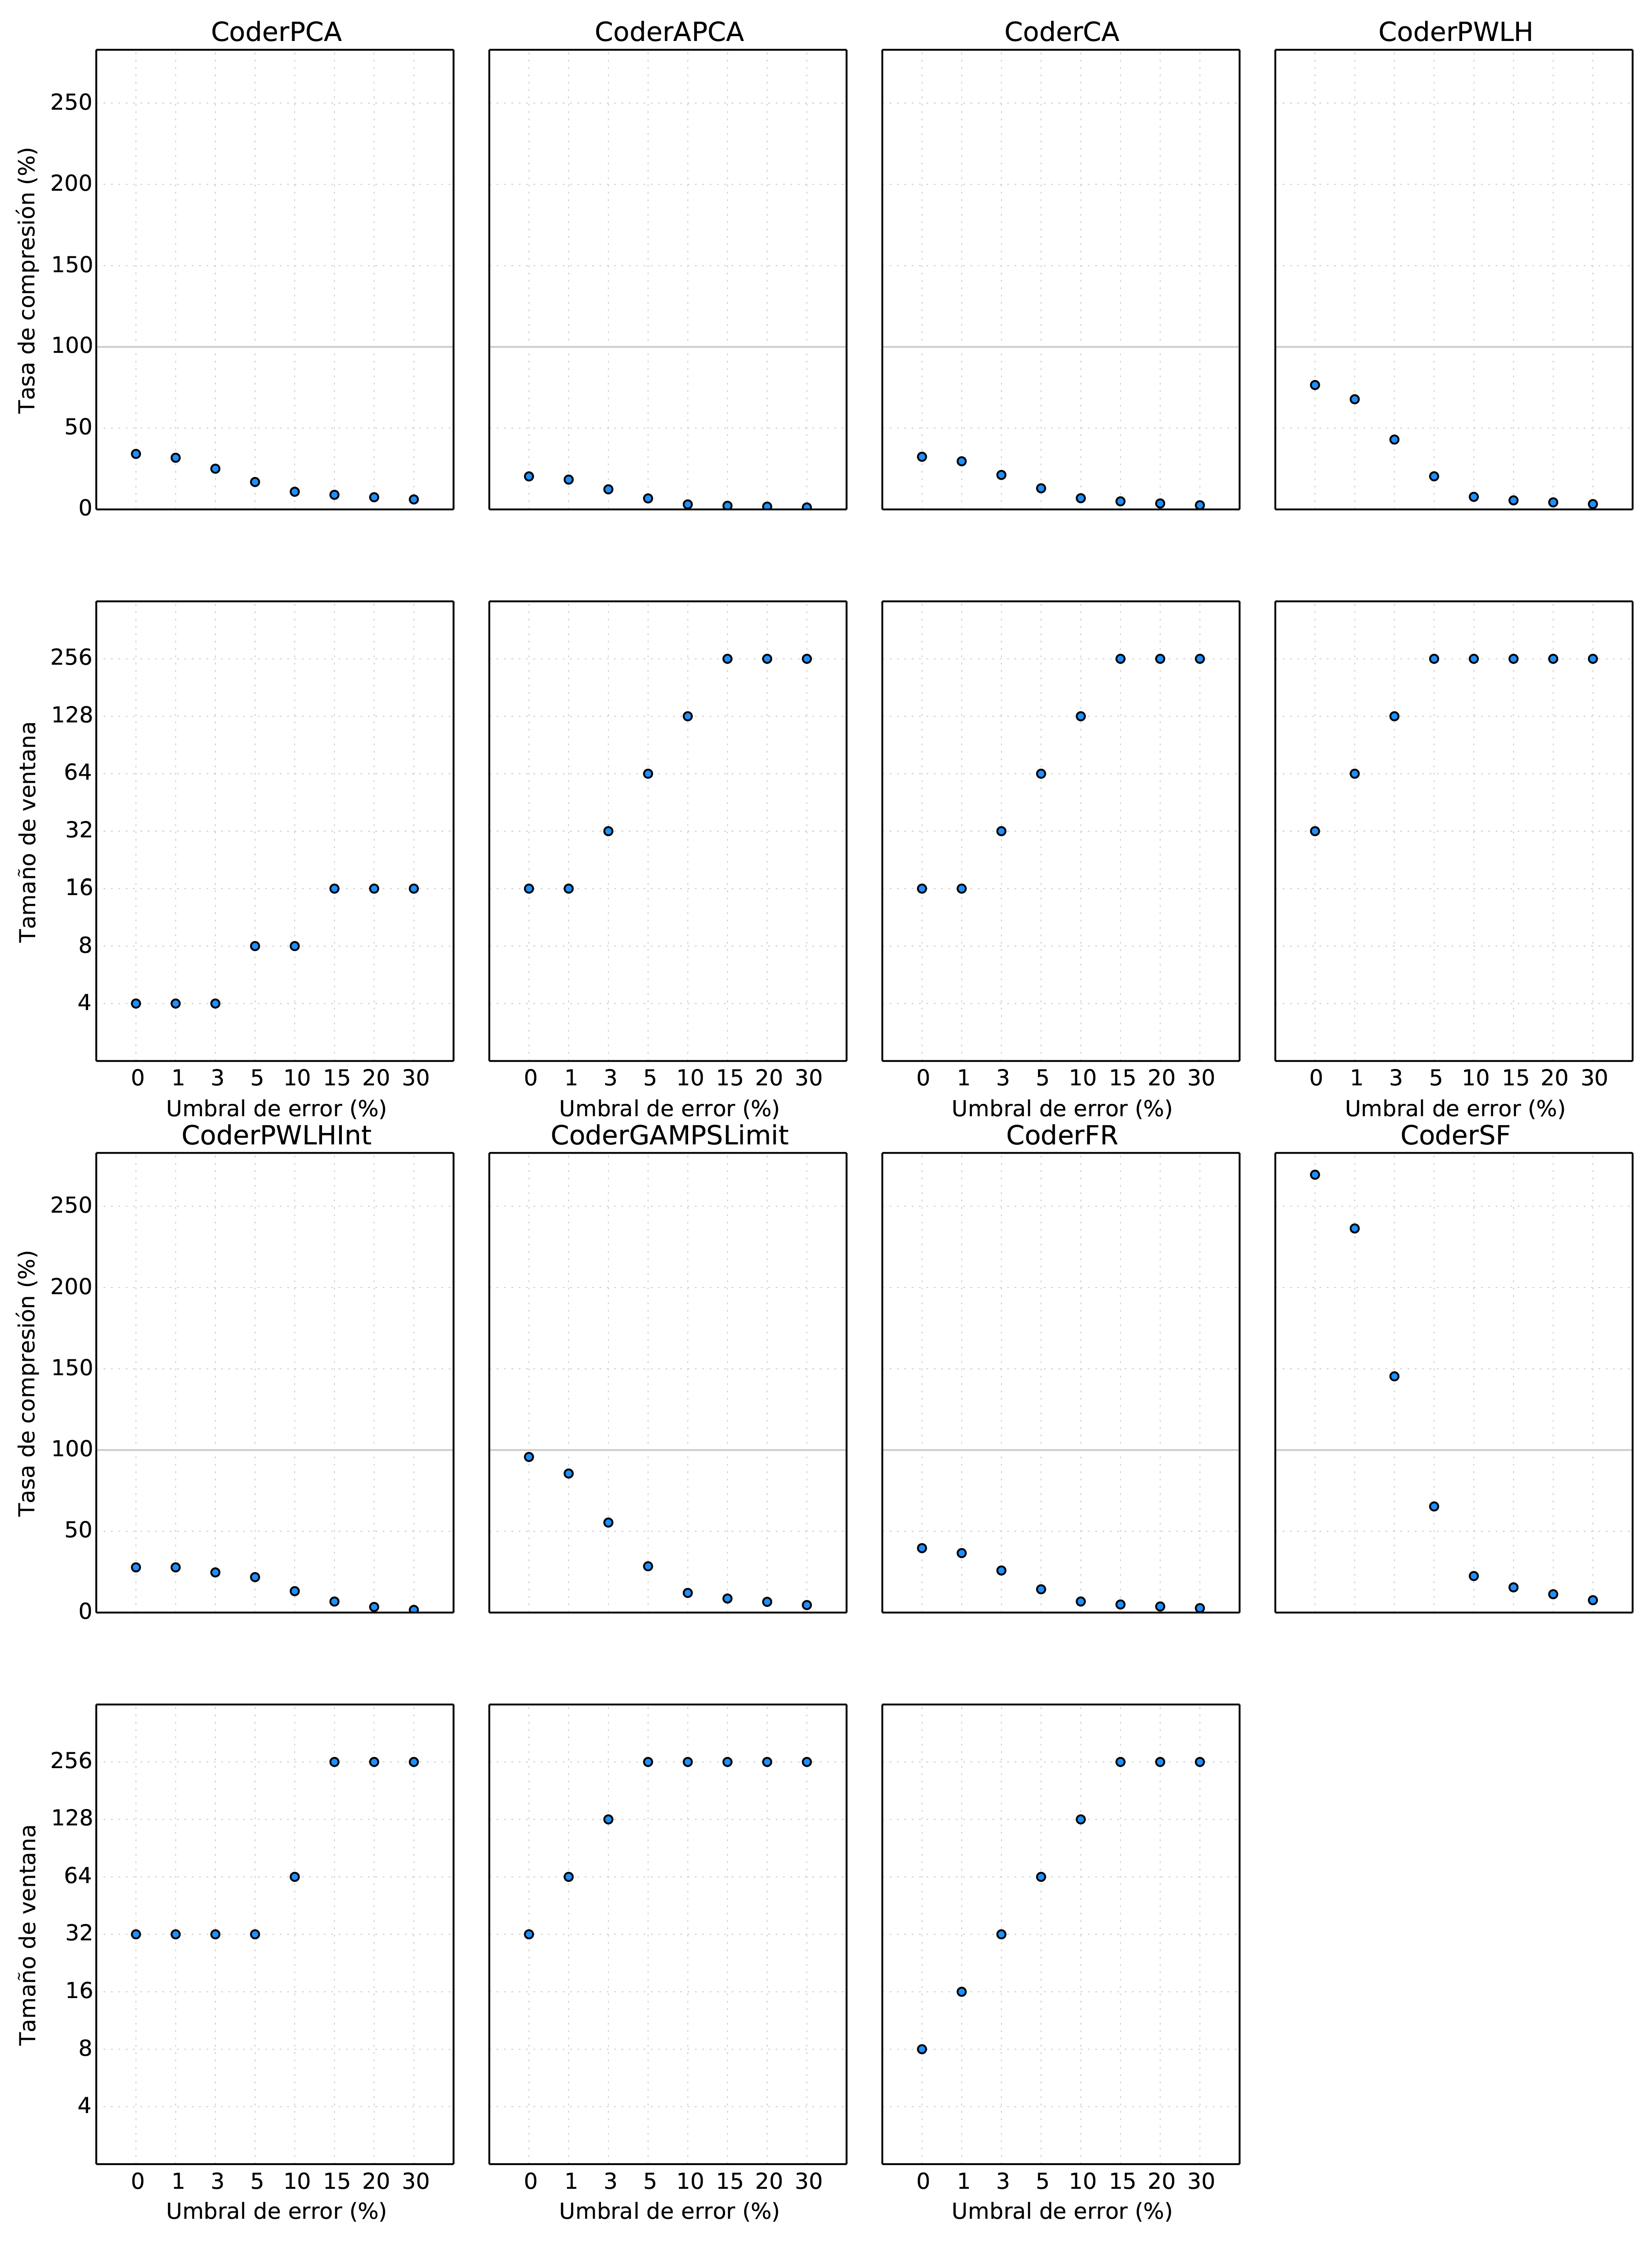
\includegraphics[scale=0.50]{chapters/Experiments/images/1-IRKIS.png}
\hspace{+10pt}
\caption{Compression rate and Window size graphs for the different combinations\\<$\coder \in C$, $w \in W, e \in E$> for the ``VWC" data type of the \datasetirkis \ dataset.}
\label{fig:mask-irkis}
\end{figure}

\clearpage







\clearpage
\section{Comparison with the gzip Algorithm}
\label{secX:gzip}
